\section{Fragen}
\subsection{Wieso ist die Annäherung für $\beta$ größer als $\pm40$ Grad nicht so gut?}
Zwischen $\beta=+40$ Grad und $\beta=-40$ Grad gibt es keine starken horizontalen Abweichungen bei der Bewegung des schwarzen Stabs. Die Bewegung ist hauptsächlich vertikal. Diese Bewegung kann linear gut approximiert werden. Nimmt $\beta$ Werte größer $40$ Grad, beziehungsweise kleiner $-40$ Grad an, wird die horizontale Auslenkung des schwarzen Stabs größer und die Approximation $\alpha=\frac{a_1}{a_2}\beta$ weicht immer stärker von der tatsächlichen Kurve $\alpha = f(\beta)$ ab. Der Graph verdeutlicht dies anschaulich.\\
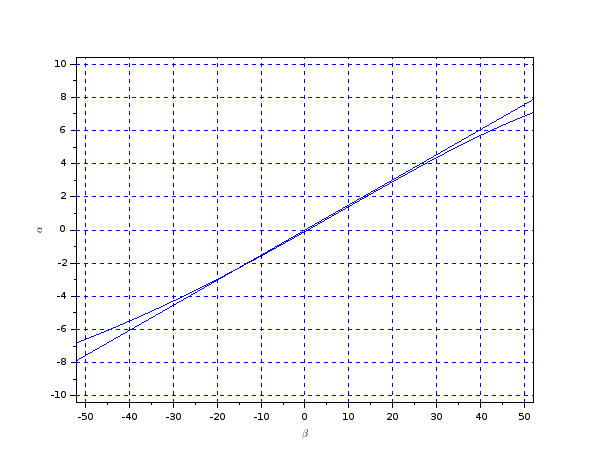
\includegraphics[scale=0.5]{images/plot1.png}

\subsection{$\beta = \pm 300$ Grad}
Wenn der Bereich von $\beta$ auf $\beta=\pm300$ Grad vergrößert wird, beginnt der Graph sich periodisch zu wiederholen, da der Servomotor den Arm auf einer Kreisbahn bewegt. Es ist also sinnlos Winkel größer als $90$ Grad, bewiehungsweise kleiner als $-90$ Grad zu betrachten, da sich die Werte nur wiederholen. \\
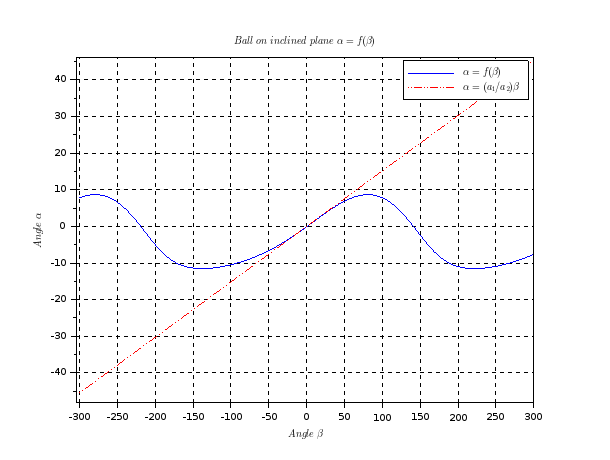
\includegraphics[scale=0.5]{images/plot2.png}

\subsection{Schwarzer Arm länger oder kürzer}
Bei einem längeren Arm und sonst gleichbleibenden Parametern, hätte die Fläche bei $\beta = 0$ Grad ein Gefälle von links nach rechts. Bei einer zu hohen Länge kann es passieren, dass sich die Fläche nur noch in dem Grad des Gefälles von links nach rechts variieren lässt, die Gegenrichtung also nicht mehr erreicht werden kann. \\
Bei einem kürzeren Arm wäre die Fläche bei $\beta = 0$ Grad auch nicht in der Waage. Es gäbe ein Gefälle von rechts nach links. Würde der Arm eine bestimmte Kürze unterschreiten, kann es passieren, dass keine Drehung des Motors mehr möglich ist, da es hängen bleibt. \\
Die Länge des Arms sollte so gewählt sein, dass die Fläche bei $\beta = 0$ Grad in der Waage ist. Somit ist gewährleistet, dass alle Positionen angefahren werden können.